% TalentScout v2 -- paper draft (Springer LNCS format).
% Compile on Overleaf or with: pdflatex main && bibtex main && pdflatex main && pdflatex main
% The llncs class and the splncs04 bibliography style ship with TeX Live and Overleaf.
\documentclass[runningheads]{llncs}

\usepackage[T1]{fontenc}
\usepackage{graphicx}
\usepackage{booktabs}
\usepackage{amsmath}
\usepackage{amssymb}
\usepackage{url}
\usepackage[hidelinks]{hyperref}

\begin{document}

\title{When Validation Gains Do Not Transfer: Nature-Inspired Feature Selection for Football Talent Identification}
\titlerunning{Nature-Inspired Feature Selection for Football Talent Identification}

\author{Roopak Raam}
\authorrunning{R. Raam}
\institute{Lovely Professional University, Phagwara, Punjab, India}

\maketitle

\begin{abstract}
A scout cannot measure every attribute of every young player, so a small attribute set that predicts future success would be valuable. We use ten seasons of EA Sports FIFA and FC ratings (FIFA~15 to FC~24) to predict which outfield players aged 21 or under and rated below 80 reach 80+ within three game versions, and we search the $2^{45}$ subsets of the game's attributes with a Genetic Algorithm, Binary PSO and a Binary Grey Wolf Optimizer under an equal budget of 600 wrapper evaluations, shared starting populations and ten seeds. The data are split by season and grouped by player, and the newest season is used once, as a test set. All three metaheuristics beat random search on every seed (Wilcoxon, Holm-adjusted $p = 0.012$) and do not differ significantly from each other; Binary GWO converged fastest and kept the fewest attributes. On validation, the selected subsets scored far above all 45 attributes (PR-AUC 0.61--0.63 against 0.50). On the test season every model scored 0.28--0.35, subsets matched the full set within noise, and no model beat EA's own potential rating for the 80+ target, although LightGBM did for a 75+ target. We trace the gap to a validation set made easier by the grouping rule and to selection fitting noise; selecting by grouped cross-validation on the training seasons did no better. We also show that the inertia schedule usually recommended for continuous PSO stops binary PSO from converging.

\keywords{Feature selection \and Genetic algorithm \and Binary particle swarm optimization \and Grey wolf optimizer \and Talent identification \and Football analytics}
\end{abstract}

\section{Introduction}

Clubs sign teenagers on a few seasons of evidence, and machine learning for talent identification is growing quickly, but a recent review of 27 team-sport studies rated 59\% at high risk of bias, mainly for leakage, missing calibration and the absence of external validation~\cite{tang2026review}. EA Sports' FIFA series offers an unusually complete alternative data source: every licensed professional is rated each season on an overall scale and about 45 attributes. Following the same players across ten launch-day snapshots lets us ask a concrete question: \emph{will a player aged 21 or under and rated below 80 reach 80+ within the next three game versions?}

Two practical goals follow. A model should rank young players better than EA's own \texttt{potential} rating, and, because a scout cannot measure 45 attributes for every youth player, a much smaller attribute set should predict as well as all of them. The second goal is a binary optimization problem with $2^{45} \approx 3.5 \times 10^{13}$ candidate solutions, the classical setting for evolutionary and swarm feature selection~\cite{xue2016survey}.

We make four contributions: (i)~a leakage-controlled benchmark for future-elite prediction with a temporal, player-grouped split and an untouched test season; (ii)~a fair comparison of a Genetic Algorithm, Binary PSO and Binary GWO for wrapper feature selection, with shared starting populations, an equal evaluation budget, ten seeds and nonparametric tests~\cite{derrac2011tutorial}; (iii)~evidence that large validation gains from feature selection vanished on the test season, with a decomposition of why and a cross-validation fallback; and (iv)~a simple explanation of why the falling inertia weight of continuous PSO disables binary PSO.

\section{Related Work}

Feldman~\cite{feldman2025predict} used FIFA ratings from 2008--2016 to predict whether players fulfil the potential the game assigned them, reaching a ROC-AUC of 0.79 with early-career data and random 5-fold cross-validation. FIFA data have also served market-value prediction, including PSO-based feature selection for support vector regression~\cite{behravan2021value}, and position classification~\cite{alasadi2021fifa}. Unlike these, we use an absolute target (80+), treat EA's potential as a baseline rather than part of the label, and evaluate on a later season. Genetic algorithms and binary PSO are the most studied evolutionary feature selectors~\cite{xue2016survey}; Emary et al.~\cite{emary2016bgwo} introduced binary GWO variants and compared them with GA and PSO on UCI data. We found no comparison of the three for talent identification.

\section{Data and Problem}

\textbf{Data and label.} The Kaggle \emph{EA Sports FC 24 Complete Player Dataset}~\cite{leone2023dataset} holds 180,021 player-versions from FIFA~15 to FC~24, one launch-day snapshot per version. A row at version $t$ is eligible if the player is 21 or younger and rated below 80, and positive if
\begin{equation}
y_{i,t} = \mathbf{1}\Big[\max_{k \in \{1,2,3\}} \mathrm{overall}_{i,t+k} \ge 80\Big].
\end{equation}
Feature rows therefore come from FIFA~15--21. Goalkeepers are removed, and players absent from all three future versions (22.6\% of eligible rows, usually players who left the licensed leagues) are dropped, leaving 22,315 labelled rows with 572 positives.

\textbf{Split.} FIFA~15--18 train the models, FIFA~19--20 validate them and FIFA~21 tests them (Fig.~\ref{fig:design}); every test player is removed from training and validation. The sets hold 12,148, 3,974 and 3,288 rows with 344, 113 and 72 positives.

\begin{figure}[t]
\centering
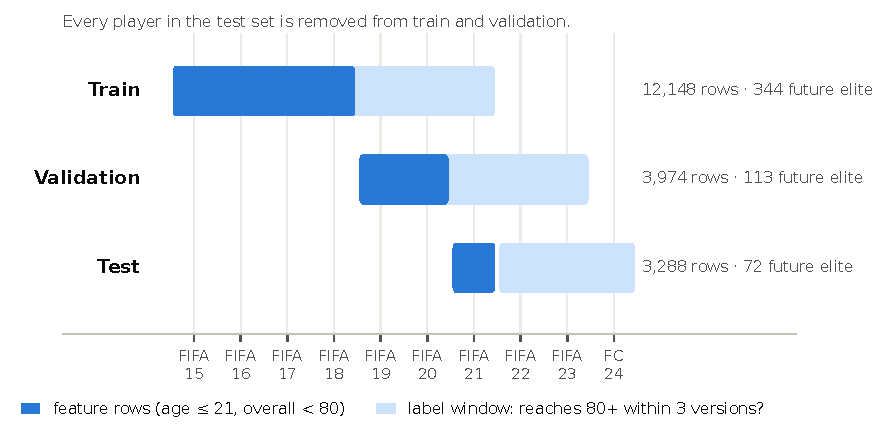
\includegraphics[width=0.92\textwidth]{figures/fig00_study_design.pdf}
\caption{Study design: feature rows (dark) and the three-version label windows (light) of each set.}
\label{fig:design}
\end{figure}

\textbf{Features and formulation.} The candidate pool has $D = 45$ attributes: current overall, profile attributes (age, height, weight, foot, weak foot, skill moves, league level, position group, one-year change in overall), six summary statistics and 29 detailed skills. EA's potential, market value, wage, release clause and reputation are kept out of the pool. A solution $\mathbf{x} \in \{0,1\}^{45}$ is scored by
\begin{equation}
f(\mathbf{x}) = \alpha\,\big(1 - \mathrm{PRAUC}_{\mathrm{val}}(\mathbf{x})\big) + (1-\alpha)\,\frac{|\mathbf{x}|}{45}, \qquad \alpha = 0.99,
\label{eq:fitness}
\end{equation}
where $\mathrm{PRAUC}_{\mathrm{val}}$ is the validation PR-AUC of a LightGBM model~\cite{ke2017lightgbm} with fixed settings (200 trees, learning rate 0.05, class weights) trained on the selected columns. An evaluation takes about 0.23\,s; every subset is cached.

\section{Methods}

\textbf{Optimizers.} The GA uses tournament selection ($k=3$), uniform crossover (0.9), bit-flip mutation ($1/D$) and two elites. Binary PSO~\cite{kennedy1997binary} draws $x_{ij} = 1$ with probability $\sigma(v_{ij})$, with $c_1 = c_2 = 2$ and velocities clamped to $\pm 6$. Binary GWO uses the bGWO2 update~\cite{emary2016bgwo}: the mean of the three leader-guided moves of GWO~\cite{mirjalili2014gwo} is passed through $\sigma(10(x - 0.5))$ and thresholded at random; $a$ falls from 2 to 0. Random search is the control. All four share one interface: for seed $s$ the starting population of 20 random vectors is identical across methods, the budget is 600 evaluations with every call counted (cache hits included), and seeds 0--9 are run.

\textbf{The inertia weight of binary PSO.} The usual continuous-PSO schedule, $w$ falling from 0.9 to 0.4~\cite{shi1998inertia}, failed a toy problem with a known optimum (minimise the number of selected bits): the swarm stalled at about 7 features and stayed almost as diverse as a random population. When a bit agrees with both the personal and the global best, the attraction terms vanish and the update is $v \leftarrow w v$; with $w < 1$ the velocity decays to 0, which in binary PSO means $P(x = 1) = 0.5$. A falling weight thus randomises the swarm over time. With $w = 1$, the original binary PSO, the optimum was reached on 10 of 10 seeds. We use $w = 1$ and report the planned schedule as an ablation. On the toy problem and on Breast Cancer Wisconsin, all three methods matched or beat random search on every seed before any football run.

\textbf{Models and tuning.} EA potential (used directly as a score), L2 logistic regression, a random forest, LightGBM and a GPU-trained MLP were tuned with 50 trials of Optuna's TPE sampler~\cite{akiba2019optuna,bergstra2011tpe} on validation PR-AUC.

\textbf{Test protocol.} Before using the test set we fixed five configurations: all 45 features; for each optimizer, the subset of its run with the best validation fitness; and the top-$k$ features by validation SHAP~\cite{lundberg2017shap}, with $k$ the median optimizer subset size ($k = 20$). Each received its own TPE-tuned LightGBM, fitted on the training rows only. Test metrics are PR-AUC with 1,000-sample bootstrap intervals, paired bootstrap differences, precision@50 and Brier scores. Optimizers were compared with a Friedman test and Holm-corrected Wilcoxon signed-rank tests~\cite{derrac2011tutorial,holm1979}.

\section{Results}

\subsection{Comparing the optimizers on validation}

Table~\ref{tab:rq2} summarises the 40 runs. Each metaheuristic beat random search on all ten seeds ($p = 0.002$, Holm-adjusted 0.012); the Friedman test rejects equal performance ($\chi^2 = 19.9$, $p = 1.8 \times 10^{-4}$), but no pairwise difference among the metaheuristics survives correction (Holm $p \ge 0.39$). They differ in how they search (Fig.~\ref{fig:conv}): all three pass random search's final value within 85 evaluations, the GA then flattens, and Binary GWO's pack collapses onto near-identical solutions (mean Hamming distance 1.6 at the end), while Binary PSO keeps exploring (7.7) and trains a new model for 595 of its 600 calls. Binary GWO keeps significantly fewer features than the GA and Binary PSO (Holm $p = 0.023$ and $0.039$). Stability is low for all methods: two runs of the same algorithm share a mean Jaccard similarity of 0.39--0.44. The planned PSO inertia schedule lost to $w = 1$ on all ten seeds ($p = 0.002$).

\begin{table}[t]
\centering
\caption{Best solution per run, mean $\pm$ sd over ten seeds (validation, fixed fitness settings).}
\label{tab:rq2}
\small
\begin{tabular}{lcccc}
\toprule
Method & Fitness & Val.\ PR-AUC & Features & Mean Jaccard \\
\midrule
GA & $0.389 \pm 0.019$ & $0.612 \pm 0.019$ & 22.1 & 0.41 \\
Binary PSO & $0.380 \pm 0.011$ & $0.621 \pm 0.011$ & 21.6 & 0.44 \\
Binary GWO & $\mathbf{0.373 \pm 0.007}$ & $\mathbf{0.627 \pm 0.007}$ & \textbf{17.9} & 0.39 \\
Random search & $0.426 \pm 0.007$ & $0.575 \pm 0.008$ & 23.7 & 0.39 \\
All 45 features & 0.506 & 0.499 & 45 & -- \\
\bottomrule
\end{tabular}
\end{table}

\begin{figure}[t]
\centering
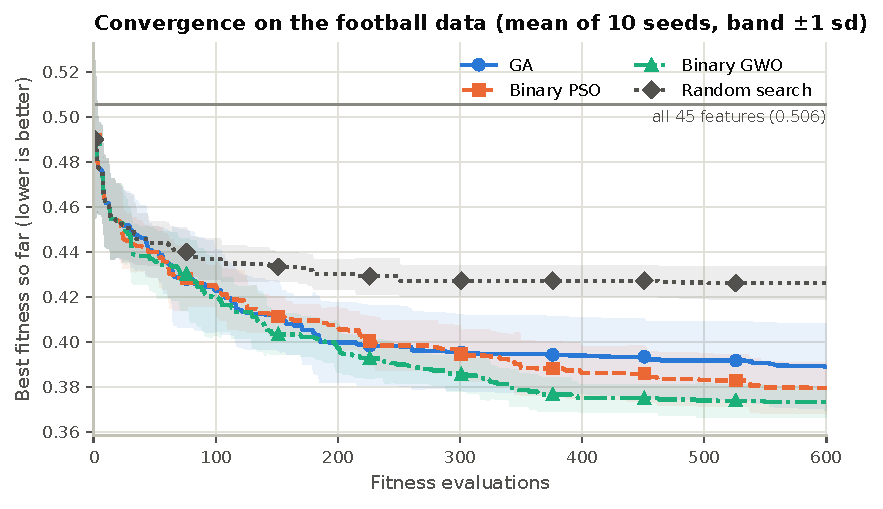
\includegraphics[width=0.49\textwidth]{figures/fig04a_convergence.pdf}\hfill
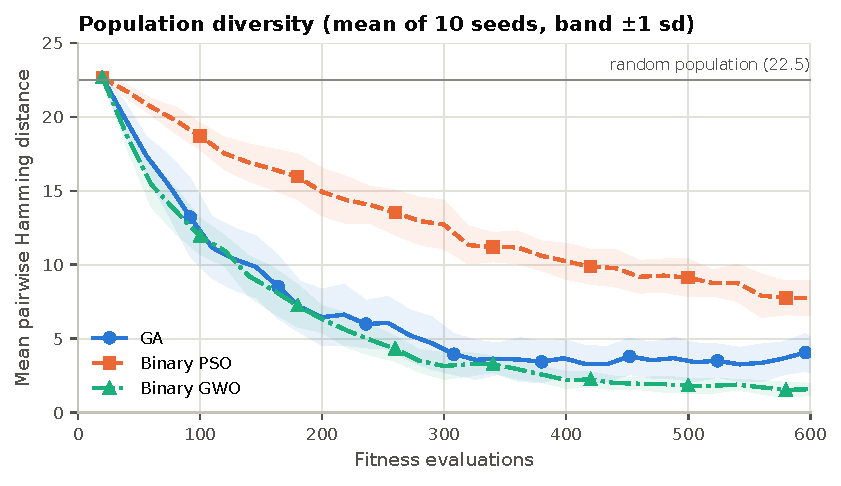
\includegraphics[width=0.49\textwidth]{figures/fig04b_diversity.pdf}
\caption{Left: best fitness so far against evaluations. Right: population diversity (mean pairwise Hamming distance). Means of ten seeds with $\pm 1$ sd bands.}
\label{fig:conv}
\end{figure}

At $\alpha = 0.99$ no run reached 15 features or fewer, because a feature costs only $0.01/45$ of fitness. Re-running Binary GWO with $\alpha \in \{0.95, 0.90, 0.80\}$ gave subsets of 8--15 features with validation PR-AUC 0.62--0.64. Over all 30,132 subsets evaluated in the study, the best validation PR-AUC rises steeply up to about nine features and is flat beyond (Fig.~\ref{fig:front}).

\begin{figure}[t]
\centering
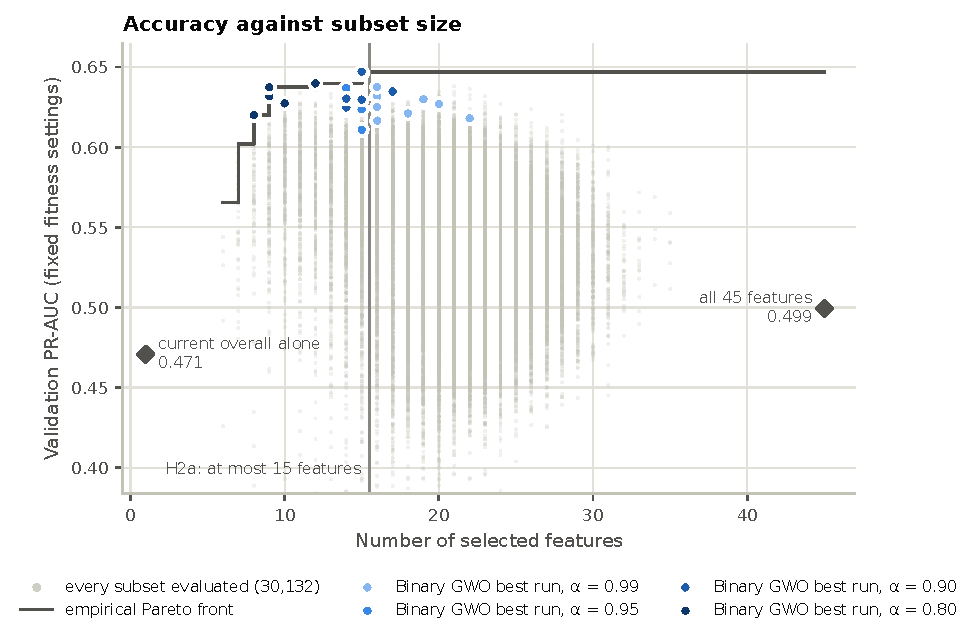
\includegraphics[width=0.82\textwidth]{figures/fig04c_tradeoff_front.pdf}
\caption{Validation PR-AUC against subset size for every evaluated subset, the empirical Pareto front and the Binary GWO runs of the $\alpha$ sweep.}
\label{fig:front}
\end{figure}

\subsection{The test season}

Table~\ref{tab:test} gives the test results. Every configuration lands between 0.28 and 0.35 PR-AUC (a random ranking scores 0.022), and no paired difference is significant. LightGBM minus EA potential is $-0.026$ [$-0.116$, $0.059$], LightGBM minus the MLP $-0.006$ [$-0.090$, $0.084$], and every subset differs from all 45 features by less than 0.02 with an interval containing zero. EA potential's top 50 contains 28 of the 72 future elite players, more than any model's. For a 75+ label, however, LightGBM beats EA potential by $+0.080$ [$+0.036$, $+0.126$]. Raw class-weighted probabilities are poorly calibrated; Platt scaling fitted on validation brings every Brier score (0.017--0.019) below the base-rate forecast (0.0214).

\begin{table}[t]
\centering
\caption{Test season (FIFA 21; 72 positives of 3,288). PR-AUC with 95\% bootstrap intervals.}
\label{tab:test}
\small
\begin{tabular}{lccc}
\toprule
Configuration & Validation PR-AUC & Test PR-AUC [95\% CI] & Precision@50 \\
\midrule
EA potential & 0.423 & 0.327 [0.233, 0.446] & 0.56 \\
Random forest & 0.539 & 0.353 [0.254, 0.482] & 0.44 \\
MLP & 0.573 & 0.307 [0.222, 0.419] & 0.36 \\
LightGBM, all 45 features & 0.593 & 0.301 [0.205, 0.420] & 0.44 \\
LightGBM, GA subset (20) & 0.636 & 0.296 [0.209, 0.422] & 0.36 \\
LightGBM, Binary PSO subset (21) & 0.650 & 0.313 [0.222, 0.435] & 0.42 \\
LightGBM, Binary GWO subset (16) & 0.624 & 0.284 [0.207, 0.405] & 0.48 \\
LightGBM, SHAP top-20 & 0.592 & 0.291 [0.204, 0.403] & 0.40 \\
\bottomrule
\end{tabular}
\end{table}

\subsection{Why the validation gains vanished}

Even EA potential, which involves no fitting, drops from 0.42 on validation to 0.33 on test, so part of the gap lies in the sets themselves. Removing every test player from validation removes exactly the players still young and below 80 in FIFA~21. On the FIFA~19--20 rows removed for that reason, EA potential scores 0.21 and the tuned LightGBM 0.19; on the rows kept in validation, 0.42 and 0.59. The kept positives were already close to the threshold (63\% rated 75+, against 46\% in test). Grouped 3-fold cross-validation within the training seasons was far more honest: all 45 features score 0.320 there and 0.312 on test, against 0.499 on validation.

The selected subsets lost about 0.05 more PR-AUC than all 45 features between validation and test, the selection bias known from other domains~\cite{ambroise2002selection,cawley2010overfitting}. Following the plan's fallback, we re-ran the three optimizers with the cross-validation fitness (seeds 0--3). Those subsets scored 0.365--0.372 in the cross-validation that chose them (all features: 0.320) but 0.280 on test, against 0.295 for the validation-chosen subsets and 0.312 for all features (Mann--Whitney $p = 0.25$). With 113--344 positives, the PR-AUC differences an optimizer chases are as large as the noise, whichever data it looks at.

\subsection{Interpretation}

Age was kept in all 30 main runs, height in 29, but current overall in only 15, although it ranks fourth by SHAP: a linear model recovers 82\% of its variance from the other attributes, so a wrapper can drop it. Selection frequency and mean $|$SHAP$|$ agree only weakly (Spearman $\rho = 0.31$). The model's best test call (Sandro Tonali, 77 at 20, later 86) and its worst miss (Randal Kolo Muani, 64 at 21, later 84) show its limit: it recognises players already near elite level, but not late development.

\section{Discussion and Limitations}

As optimizers, all three metaheuristics did their job, and the choice among them mattered less than giving each a fair budget. As a predictor, no attribute set beat EA's judgement for the 80+ target, which draws on match information the card lacks; compact subsets, however, lose nothing measurable, so a scouting checklist can be cut to a third or half of the attributes. The main methodological lesson is that wrapper selection with few positives will always find subsets that look better on the data it is shown; only untouched data can tell the difference, and the validation set must resemble the test set, which a grouping rule can quietly prevent. Limitations: labels and features are both EA ratings; only one test season (72 positives) was available; only licensed leagues and outfield players are covered; the fitness used fixed LightGBM settings; and the $\alpha$ sweep covered Binary GWO only.

\section{Conclusion}

Nature-inspired optimizers reliably beat random search for feature selection on football talent data, but their validation gains did not transfer to a later season. Future work includes NSGA-II for a true multi-objective front, stability-aware selection, tuning and selection by grouped cross-validation over several seasons, and match and injury data.

\bibliographystyle{splncs04}
\bibliography{references}

\end{document}
